\documentclass[output=paper]{langsci/langscibook} 
\author{%
	Andy Lücking\affiliation{Goethe-Universität Frankfurt}%
	\and Jonathan Ginzburg\affiliation{Université de Paris}%
	\lastand Robin Cooper\affiliation{G\"{o}teborgs Universitet}%
}
% \title{Pragmatics and dialogue semantics}
\title{Grammar in dialogue}

% \chapterDOI{} %will be filled in at production

\epigram{\enquote{It takes two to make a truth.}\\ \citet[\page 124, fn.~1]{Austin:1950}}

\abstract{This chapter portrays some phenomena, technical developments and discussions that are pertinent to analysing natural language use in face-to-face interaction from the perspective of HPSG and closely related frameworks.
%
The use of the \textsc{context} attribute in order to cover basic pragmatic meaning aspects is sketched.
%
With regard to the notion of common ground it is argued how to complement \textsc{context} by a dynamic update semantics.
%
Furthermore, this chapter discusses challenges posed by dialogue data such as clarification requests to unification-based, model-theoretic grammars.
%
Responses to these challenges in terms of a type-theoretical underpinning (TTR, a Type Theory with Records) of both the semantic theory and the grammar formalism are reviewed.
%
Finally, the dialogue theory \emph{KoS} is sketched that emerged in this way from work in HPSG.
}

\maketitle

\begin{document}
\label{chap-pragmatics}

{
\avmoptions{}
%\avmfont{\footnotesize}
%\avmsortfont{\itshape}


\section{Introduction} 
\label{sec:introduction}

The archaeologists Ann Wesley and Ray Jones are working in an excavation hole, Ray Jones is looking at the excavation map.
%
Suddenly, Ray discovered a feature that catches his attention. %
He turns to his colleague Ann and initiates the following exchange (the example is slightly modified from \citet[\page 222]{Goodwin:2003}; underlined text is used to indicate overlap, italic comments in double round brackets are used to describe non-verbal actions, numbers in brackets quantify the duration of pauses):
%
\ea \label{ex:ann-ray}
\begin{enumerate}[noitemsep]
    \item \speaking{Ray:} Doctor Wesley?
    \item \speaking{} \quad (0.7) ((\textit{Ann turns and walks towards Ray}))
    \item \speaking{Ann:} EHHH HEHH ((\textit{Cough}))
    \item \speaking{} Yes Mister Jones.
    \item \speaking{Ray:} I was gonna see:
    \item \speaking{Ann:} \textdegree Eh heh huh huh
    \item \speaking{} \eqparbox{eh}{\textdegree eh heh} \underline{huh huh}
    \item \speaking{Ray:} \eqparbox{eh}{\ } \underline{Uh::m},
    \item \speaking{Ann:} Ha huh HHHuh
    \item \speaking{Ray:} ((\textit{Points with trowel to an item on the map})) \\ 
    \speaking{} I think I finally found \textbf{this} feature \\
    \speaking{} ((\textit{looks away from map towards a location in the}\\ \speaking{} \textit{surrounding}))
    \item \speaking{} (0.8) Cause I: hit the \textbf{nai}l
    \item ((\textit{Ann looks at map, Ray looks at Ann, Ann looks at Ray}))
\end{enumerate}
\z


Contrast the archaeological dialogue from (\ref{ex:ann-ray}) with a third person perspective text on a related topic.
%
In a recent archaeology paper, the excavation of gallery grave Falk\"{o}ping stad 5 is described, among others \citep[\page 4]{Blank:Tornberg:Knipper:2018}:
%
\begin{quote}
During excavation the grave was divided in different sections and layers and the finds were documented in these units. The bone material lacking stratographic and spatial information derives from the top layer [\ldots]. Both the antechamber and the chamber contained artefacts as well as human and animal skeletal remains, although most of the material was found in the chamber.
\end{quote}


The differences between the archaeological dialogue and the paper are obvious and concern roughly the levels of \emph{medium} \is{medium} (spoken vs. written), \emph{situatedness} \is{situatedness} (degree of context dependence), \emph{processing speed} \is{processing speed} (online vs. offline), and \emph{standardisation} \is{standardisation} (compliance with standard language norms) \citep{Klein:1985}.
%
Attributing differences between dialogue and text simply to the medium (i.e. spoken vs. written) is tempting but is insufficient. 
%
The corresponding characterising features seem to form a continuum, as discussed under the terms \emph{conceptual orality} \is{conceptual orality} and \emph{conceptual literacy} \is{conceptual literacy} in the (mainly German speaking) literature for some time \citep{Koch:Oesterreicher:1985}.
%
For example, much chat communication, although realised by written inscriptions, exhibits many traits of (conceptually) spoken communication, as investigated, for instance, by means of chat corpora \citep{Beisswenger:et:al:2012:a}. 
%
Face-to-face dialogue stands out due to a high degree of \isi{context dependence} manifested in \isi{shared attention} (\citet{Tomasello:1998}; see also turns 2 and 12 between Ann and Ray), \isi{non-verbal actions} such as hand and arm gestures (\citet{Kendon:2004,McNeill:2000:a}; turn 10; cf. \crossrefchaptert{gesture} for a brief overview of non-verbal communication means), \isi{disfluencies} (\citealp{Ginzburg:Fernandez:Schlangen:2014}; turn 5 to 8), \isi{non-sentential utterances} (\citealp{Fernandez:Ginzburg:2002,Fernandez:Ginzburg:Lappin:2007}; turns 1, 4, and 5), \isi{laughter} (\citealp{Ginzburg:Breitholz:Cooper:Hough:Tian:2015}; turn 9), \isi{shared knowledge} of interlocutors (\citealp{Clark:Schreuder:Buttrick:1983}; turns 10--12), \isi{turn-taking} (\citealp{Sacks:Schegloff:Jefferson:1974,heldner2010,levinson2015}; e.g. question-answering in turns 1 and 4), \isi{indirect reference} (turn 10, where Ray points to an item on the map but refers to an archaeological artefact in the excavation hole). Such instances of \isi{deferred reference} \citep{Nunberg:1993} in \isi{situated communication} actually differ from \isi{bridging} anaphora \citep{Clark:1975} in written texts (cf. \citealp{Luecking:2018:a}).

\is{linguistic knowledge|(}
Since these phenomena are usually abstracted away from the linguistic knowledge encoded by a grammar, linguistics is said to exhibit a \enquote{written language bias} \is{written language bias} \citep{Linell:1982}.
%
In fact, many of the phenomena exemplified above provide serious challenges  to current  linguistic theory, as has been argued by \citet{Ginzburg:2012}, \citet{Ginzburg:Poesio:2016} and \citet{Kempson:Cann:Gregoromichelaki:Chatzikyriakidis:2016}.
%
\is{language system|(}
So the question is: how serious is this bias? 
%
Is there a single language system with two modes, written and spoken (but obeying the qualifications we made above with respect to conceptual orality and literacy)?
%
Or do written and spoken communication even realise different language systems?
%
Responses can be given from different standpoints. 
%
When the \isi{competence}/""\isi{performance}  distinction was proposed \citep{Chomsky:1969}, one could claim that linguistic knowledge is more purely realised by the high degree of standardisation manifested in written text, while speech is more likely to be affected by features attributed to performance (e.g.,  processing issues such as short term memory limitations or impaired production/""perception).
%
Once one attaches more importance to dialogical phenomena, one can also claim that there is a single, basic language system underlying written and spoken communication which bifurcates only in some cases, with interactivity and deixis being salient examples (such a position is delineated but not embraced by \citet{Klein:1985}; in fact, Klein remains neutral on this issue). 
%
Some even claim that \enquote{grammar is a system that characterizes talk in interaction} \citep[\page 1]{Ginzburg:Poesio:2016}. 
%
This position is strengthened by the primacy of spoken language in both ontogenetic and language acquisition areas (on acquisition see \crossrefchaptert{acquisition}).
\is{language system|)}

Advances in dialogue semantics are compatible with the latter two positions, but their ramifications are inconsistent with the traditional competence/""performance distinction \citep{Ginzburg:Poesio:2016,Kempson:Cann:Gregoromichelaki:Chatzikyriakidis:2016}. 
%
Beyond investigating phenomena which are especially related to people engaging in face-to-face interaction, dialogue semantics contributes to the theoretical (re-)""consideration of the \isi{linguistic competence} that grammars encode.
%
Some of the challenges posed by dialogue for the notion of linguistic knowledge -- exemplified by non-sentential utterances such as clarification questions and reprise fragments \citep{Fernandez:Ginzburg:2002,Fernandez:Ginzburg:Lappin:2007} -- are also main actors in arguing \emph{against} doing semantics within a unification-based framework (Section~\ref{sec:sub-sentential-meanings} below).
\is{linguistic knowledge|)}
%
In light of this, the relevant arguments are briefly reviewed below.
%
Subsequently, TTR (a Type Theory with Records) is briefly introduced in Section~\ref{sec:brief-primer-ttr}. TTR is a strong competitor to other formalisms since it provides an account of semantics that covers dialogue phenomena from the outset.
%
TTR also allows for \enquote{emulating} an HPSG kind of grammar, giving rise to a unified home for sign-based \textsc{synsem} interfaces bridging to dialogue gameboards (covered in Section~\ref{sec:hpsgttr-dialogue-game-boards}).
%
To begin with, however, we give a brief historical review of pragmatics within HPSG.







\section{From \textsc{context} to update semantics for dialogue}
\label{sec:history}

HPSG's interface to pragmatics is the \textsc{context} attribute. 
%
The \textsc{context} attribute accommodates contextual constraints that have to be fulfilled in order for an expression to be used appropriately, or felicitously \citep{Austin:1962}, to use a term from speech act theory \citep[\page 27]{Pollard:Sag:1994}.
%
It has been used and extended to model the content of indexical and pronominal expressions (see Section~\ref{sec:c-inds-background}), information packaging (Section~\ref{sec:information-structure}) and shared background assumptions concerning standard meanings (Section~\ref{sec:mutual-beliefs}).
%
A further step from such pragmatic phenomena to dialogue semantics is achieved  by making signs encode their dialogue context, leading to an architectural revision in terms of \emph{update semantics} (see Section~\ref{sec:dialogue-game-boards}).


\is{circumstantial features|(} \is{background information|(}
\subsection{\textsc{c-inds} and \textsc{background}}
\label{sec:c-inds-background}
 
The \textsc{context} \isfeat{context} attribute introduces two sub-attributes, \textsc{contextual-indices} (\textsc{c-inds}) \isfeat{contextual-indices} \isfeat{c-inds} and \textsc{background}. \isfeat{background}
%
The \textsc{c-inds} attribute value provides pointers to circumstantial features of the utterance situation such as speaker, addressee, time and location of speaking.
%
Within the \textsc{background} attribute, assumptions such as presuppositions or conventional implicatures are expressed in terms of \emph{psoas}, \emph{parameterised state of affairs} (see Section~\ref{sec:semantic-objects} for some alternative semantic representation formats). 
%
For instance, it is part of the background information of the \isi{pronoun} \textit{she} of the \enquote{natural gender language} English that its referent is female (this does not hold for \enquote{grammatical gender languages} like French or German).
%
In the HPSG format of \citet[\page 20]{Pollard:Sag:1994}, this constraint is expressed as in (\ref{ex:she}):
%
\ea \label{ex:she}
\begin{avm}
\[\asort{word} 
\textsc{phon} & /she/ \\
\textsc{synsem} & 
    \[\asort{synsem}
    \textsc{local} & 
        \[\asort{local}
        \textsc{category} & \[\asort{cat} 
                            \textsc{head} & \textit{noun}[\textsc{case} \textit{nom}] \\
                            \textsc{subcat} & \q<\quad\q>
                            \] \\
        \textsc{content} & \[\asort{ppro}  
                            \textsc{index} & \@1\[\asort{ref}
                            \textsc{per} & \textit{3rd} \\ \textsc{num} & \textit{sing} \\ 
                            \textsc{gen} & \textit{fem}
                                                \] \\
                            \textsc{restr} & \{\quad\} 
                            \] \\
        \textsc{context} & \[\asort{context}  
                            \textsc{background} & \{\[\asort{psoa}
                            \textsc{reln} & \textit{female} \\
                            \textsc{inst} & \@1
                            \]\}
                            \]
        \]
    \]
\]
\end{avm}
\z

The \textsc{content} \isfeat{content} value is of type \textit{ppro} (\textit{personal-pronoun}), which is related to the NP type ($+$p,$-$a) from \emph{Government and Binding} theory \citep{Chomsky:1981} and interacts with HPSG's binding theory (see \crossrefchaptert{binding}; see also \crossrefchaptert{agreement}).
%
The \textsc{content}/""\textsc{context} description in (\ref{ex:she}) claims that whatever the referent of the pronoun is, it has to be female.


The contextual indices that figure as values for the \textsc{c-inds} attribute provides semantic values for \isi{indexical expressions}.
%
For instance, the referential meaning of the singular \isi{first person pronoun} \textit{I} is obtained by identifying the semantic index with the contextual index \enquote{speaker} \is{speaker} (for a collection of indirect uses of \textit{I}, or rather its German cognate \textit{Ich}, where identification with the circumstantial speaker role would lead to wrong results, see \citet{Kratzer:1978}).
%
This use of \textsc{context} is illustrated in (\ref{ex:I}), which is part of the lexical entry of \textit{I} (see the \crossrefchaptert{lexicon} on the lexicalist orientation of HPSG).
%
\ea \label{ex:I}
\begin{avm}
\[\asort{word}
\textsc{phon} & /i/ \\
\textsc{synsem} & 
    \[\asort{synsem}
    \textsc{local} & 
        \[\asort{local}
        \textsc{content} & 
            \[\asort{ppro}
            \textsc{index} & \@1\[\asort{ref}
                                \textsc{ref} & \textit{1st} \\
                                \textsc{num} & \textit{sing}
                                \] \\
            \textsc{restr} & \{\} \\
            \] \\
        \textsc{context} & \[\asort{context}
                            \textsc{c-inds} & \[\asort{psoa}
                            \textsc{spkr} & \@1 \\
                            \textsc{addr} & \@2 \\
                            \textsc{time} & \@3 \\
                            \textsc{loc} & \@4
                            \]
                            \]
        \]
    \]
\]
\end{avm}
\z


Inasmuch as the  \isi{contextual anchors} (see \citet{Barwise:Perry:1983} or \citet{Devlin:1991} on anchors in situation semantics) indicated by a boxed notation from (\ref{ex:I}) provide a semantic value for the speaker in a directly referential \is{direct reference} manner (see \citet{Marcus:1961} and \citet{Kripke:1980} on the notion of direct reference with regard to proper names), they also provide semantic values for the \isi{addressee} (figuring in the content of \textit{you}), the time (\textit{now}) and the place (\textit{here}) of speaking.\footnote{Of these, in fact, only the speaker is straightforwardly given by the context; all others can potentially involve complex inference.}
%
Hence, the \textsc{context} attribute accounts for the standard indexical expressions and provides present tense marker needed for a semantic of tenses \is{tense} in the line of \emph{Discourse Representation Theory}  (\citet{Kamp:Reyle:1993}; see \citet{partee1973some} on the preeminent role of an indexical time point).
%
We will not discuss this issue further here (see \citet{Van-Eynde:1998,Van-Eynde:2000}, \citet{Bonami:2002} and \citet{Costa:Branco:2012} for HPSG work on tense and aspect), but move on to briefly recapture other phenomena usually ascribed to pragmatics (see also \citet[Sec.~5.2]{Kathol:Przepiorkowski:Tseng:2011}).
\is{circumstantial features|)} \is{background information|)}




\is{information structure|(} \is{focus|(} \is{information packaging|(}
\subsection{Information structure}
\label{sec:information-structure}

Focus, expressed by sentence accent in English, can be used for information packaging that may lead to truth-conditional differences \is{truth-conditional difference} even in case the surface structures (i.e. strings; see Section~\ref{sec:introduction} on a brief juxtaposition of spoken and written language) are the same.
%
An example is given in (\ref{ex:show-pictures}), taken from \citet[\page 246]{Krifka:2008}, where capitalisation indicates main accent and subscript \enquote{F} labels the focused constituent:
%
\ea \label{ex:show-pictures}
  \ea John only showed Mary [the PICTures]$_\text{F}$
  \ex John only showed [MARY]$_\text{F}$ the pictures.
  \z
\z


An analysis of examples like (\ref{ex:show-pictures}) draws on an interplay of phonology, semantic, pragmatic and constituency and hence emphasise in particular the advantages of the \emph{fractal} \citep{Johnson:Lappin:1999} architecture \is{fractal architecture} \is{fractality} of HPSG (see the sections on \crossrefchaptert{cg}, \crossrefchaptert{minimalism}, \crossrefchaptert{cxg}, \crossrefchaptert{lfg} and \crossrefchaptert{dg} for a comparison of HPSG to other grammar theories; a benchmark source is \citealp{Mueller:2016}).


\is{given information|(} \is{new information|(}
At the core of information structure is a distinction between \emph{given} and \emph{new} information. 
%
Accordingly, information structure is often explicated in terms of \isi{dynamic semantics} (ranging from \emph{File Change Semantics} \citep{Heim:2002} and \emph{Discourse Representation Theory} \citep{Kamp:Reyle:1993} to information state update semantics proper \citep{Traum:Larsson:2003}) -- see for instance \citet{Krifka:2008} or \citet{Vallduv`i2015} for a discussion and distinction of various notions bound up with information structure such as \emph{focus}, \emph{topic}, \emph{ground} and \emph{comment} seen from the perspective of dialogue content and dialogue management.
%
The most influential approach to information structure within HPSG is that of \citet{Engdahl:Vallduvi:1996}.
%
Here a distinction between \emph{focus}, \is{focus}\isfeat{focus} that is new information, and \emph{ground}, \is{ground}\isfeat{ground} the given information, is made \citep[\page 3]{Engdahl:Vallduvi:1996}. 
%
The \emph{ground} is further bifurcated into \textsc{link} \isfeat{link} and \textsc{tail}, \isfeat{tail} which connect to the preceding discourse in different ways (basically, the link corresponds to a discourse referent or file, the tail corresponds to a predication which is already subsumed by the interlocutors' information states).
%
The information packaging of the content values of a sentence is driven by phonetic information in terms of \isi{A-accent} and \isi{B-accent} \citep{Jackendoff:1972}, where \enquote{A-stressed} constituents are coindexed (via structure sharing, see \crossrefchaptert{formal-background}) with \textsc{focus} elements and \enquote{B-stressed} are coindexed with \textsc{link} elements -- see also \crossrefchaptert{information-structure}.
%
The \textsc{context} extension for information structure on this account is given in (\ref{ex:focus-link-tail}):
%
\ea \label{ex:focus-link-tail}
\begin{avm}
\[\asort{context}
\textsc{c-inds} & \[\quad\] \\
\textsc{backgr} & \{\quad\} \\
\textsc{info-str} & 
    \[\asort{info-struc}
    \textsc{focus} & \textit{Set}(\textit{content}) \\
    \textsc{ground} & 
        \[\asort{ground}
        \textsc{link} & \textit{Set}(\textit{content}) \\
        \textsc{tail} & \textit{Set}(\textit{content}) 
        \]
    \]
\]
\end{avm}
\z


Part of the analysis of the sample sentences from (\ref{ex:show-pictures}) is that in (\ref{ex:show-pictures}a) the content value of the indirect object NP \textit{the pictures} is the focused constituent, while it is the content value of the direct object NP \textit{Mary} in (\ref{ex:show-pictures}b).
%
The \textsc{focus-link-tail} approach entails, however, that the packages of information structure coincide with syntactic constituents.
\is{given information|)} \is{new information|)}
%
This assumption is given up in the approach to \emph{prosodic constituency} \is{prosodic constituency} of \citet{Klein:2000} -- see also \crossrefchaptert{phonology}.
%
Information structure realised by prosodic stress is also part of the speech-gesture interfaces within multimodal extensions of HPSG (cf. \crossrefchaptert{gesture}).
\is{information structure|(} \is{focus|)} \is{information packaging|)}



\subsection{Mutual beliefs}
\label{sec:mutual-beliefs}

A strictly pragmatic view on meaning and \isi{reference} is presented by \citet{Green:1996}.
%
Green provides a \textsc{context} extension for the view that restrictions on the index actually are background assumption concerning standard uses of referential expressions.
%
One of the underlying observations is that people can, for example, use the word \textit{dog} to refer to, say, toy dogs or even, given appropriate context information, to a remote control (we will come back to this example shortly).
%
The fact that the word \textit{dog} can be used without further ado successfully to refer to instances of the subspecies \textit{Canis lupus familiaris}\footnote{\label{fn:canis}\citet[Ex.~(73)]{Green:1996} actually restricts the standard use of \textit{dog} to the family \textit{Canis} (regiven in our example (\ref{ex:dog})), which seems to be too permissive. The \textit{Canis} family also include foxes, coyotes and wolves, which are, outside of biological contexts, usually not described as being dogs. This indicates that the \textsc{experiencer} group should be further restricted and allowed to vary over different language communities and genres.} is due to \isi{shared assumptions} about the \isi{standard meaning} of \textit{dog}.
%
Green represents this account in terms of \isi{mutual beliefs} between \textsc{experiencer} \isfeat{experiencer} and \textsc{standard} \isi{standard} as part of the \isi{background condition} of the \textsc{context} of \isi{referential NPs}.
%
The semantic part of the lexical structure of \textit{dog} is given in (\ref{ex:dog}).
%
The analysis of \isi{proper names} is pursued in similar manner, amounting to the requirement that for a successful use of a proper name the interlocutors have to know that the intended referent of this name actually bears the name in question.
%
\ea  \label{ex:dog}
\begin{avm}
  \[\asort{word}
    \textsc{phon} & /dog/ \\
    \textsc{content} & \[\asort{ref}
      \textsc{index} & \@1\] \\
    \textsc{context} & \[\asort{context}
      \textsc{c-inds} & \[\asort{psoa}
        \textsc{spkr} & \@2 \\
        \textsc{addr} & \@3
      \] \\
      \textsc{background} & \{
      \[\asort{mutually-believe}
        \textsc{experiencer} & \@2 \\
        \textsc{standard} & \@3 \\
        \textsc{soa} & \[\asort{normally-believe}
          \textsc{experiencer} & \textit{English speakers} \\
          \textsc{soa} & \[\asort{canis}
            \textsc{inst} & \@1\]
        \]
      \]
      \}
    \]
  \]
\end{avm}
\z

Adding beliefs to \textsc{context} provides the representational means to integrate (at least some kinds of) presuppositions, illocutionary force and deferred reference \citep{Nunberg:1978} into grammar.
%
However, a fuller model of speech acts and meaning transfers is still needed \citep[\page 94]{Kathol:Przepiorkowski:Tseng:2011}. % \footnote{On the evolution of HPSG see \crossrefchaptert{evolution}.}


\is{common ground|(}
Taking a closer look at the argument underlying adding \isi{mutual beliefs} to \textsc{context}, one notices a striking similarity of shared assumptions about standard uses with \emph{community membership} \is{community membership} as a source for common ground (but see Footnote~\ref{fn:canis} for a hint on a possible refinement).
%
However, community membership is just one of three sources of information on which the common ground between two interlocutors (scaling up to multilogue is obvious) can be based according to \citet{Clark:Marshall:1981} and \citet{Clark:Schreuder:Buttrick:1983}:
%
\begin{quote}
The first is \emph{perceptual evidence}, what the two have jointly experienced or are jointly experiencing at the moment. The second is \emph{linguistic evidence}, what the two have jointly heard said or are now jointly hearing as participants in the same conversation. The third is \emph{community membership}. They take as common ground everything they believe is universally, or almost universally, known, believed, or supposed in the many communities and subcommunities to which they mutually believe they both belong. \hfill \citep[\page 247]{Clark:Schreuder:Buttrick:1983} 
\end{quote}


Reconsidering the \enquote{\textit{dog}-used-to-refer-to-remote-control} example mentioned above: in order for this kind of reference to happen, one can imagine a preparatory sequence like the following:
%
\ea
Can you please give me the \ldots what's the name? \ldots the \ldots ah, let's call it \enquote{dog} \ldots can you please give me the dog?
\z

In this monologue, the speaker establishes a name for the remote control.
%
After this baptism, the situationally re-coined termed can be used referentially (see \citet{Luecking:Rieser:Staudacher:2006:b} on situated conventions).
%
Obviously, the felicity of reference is due to \emph{linguistic evidence} \is{linguistic evidence} provided and agreed upon in dialogical exchange.
%
Dialogue contexts and the dynamics of common ground is a dimension which is absent in the static \textsc{context} representations surveyed above.
%
This is where dynamic update semantics enters the stage.
\is{common ground|)}




\subsection{Towards an update semantics for dialogue}
\label{sec:dialogue-game-boards}

Starting from Stalnakerian contexts \is{context} (\citealp{Stalnaker:1978}; see also \citealp{Lewis:1979:b}), that is, contexts which consist of mutually known propositions (also corresponding roughly to the mutual belief structures employed by \citealp{Green:1996}, cf. Section~\ref{sec:mutual-beliefs}), Ginzburg argues in a series of works that this context actually has a more elaborate structure \citep{Ginzburg:1994,Ginzburg:1996,Ginzburg:1997}.
%
One motivation for this refinement is found in data like (\ref{ex:Cambridge}), an
example given by \citet[\page 2]{Ginzburg:1994} from the \isi{London-Lund corpus} \citep{Svartvik:1990}.
%
\ea \label{ex:Cambridge}
\begin{enumerate}[noitemsep]
\item \speaking{A:} I've been at university.
\item \speaking{B:} Which university?
\item \speaking{A:} Cambridge.
\item \speaking{B:} Cambridge, um.
\item \speaking{} what did you read?
\item \speaking{A:} History and English.
\item \speaking{B:} History and English.
\end{enumerate}
\z

There is nothing remarkable about this dialogical exchange, it is a mundane  piece of natural language interaction.
%
However, given standard semantic assumptions and  a \emph{given-new} information \is{new information} \is{given information} structuring as sketched in Section~\ref{sec:information-structure},  (\ref{ex:Cambridge}) poses two problems.
%
The first problem is that one and the same word, namely \textit{Cambridge}, plays a different role in different contexts as exemplified by turns 2 to 3 on the one hand and turns 3 to 4 on the other hand.
%
The reason is that the first case instantiates a \isi{question-answering pair}, where \textit{Cambridge} provides the requested referent.
%
The second case is an instance of \emph{accept}: \is{acceptance} speaker B not only signals that she heard what A said (what is called \emph{acknowledge}), \is{acknowledgment} but also that she updates \is{update} her \isi{information state} with a new piece of information (namely that A studied in Cambridge).

The second problem is that neither of B's turns 4 and 7 is redundant although neither of them contribute new information (or \emph{foci} in the terminology of Section~\ref{sec:information-structure}): the turns just consist of a replication of A's answer.
%
The reason for non-redundancy obviously is that in both cases the repetition manifests an \emph{accept} \is{acceptance} move in the sense just explained.


In order to make grammatical sense out of such dialogue data -- eventually in terms of \isi{linguistic competence} -- contextual background rooted in language \is{community membership} is insufficient, as discussed.
%
The additional context structure required to differentiate the desired interpretation of (\ref{ex:Cambridge}) from redundant and co-text insensitive ones is informally summarised by \citet[\page 4]{Ginzburg:1994} in the following way:
%
\begin{quote}
  \begin{itemize}
  \item \textsc{facts}: \isfeat{facts} a set of commonly agreed upon \isi{facts};
  \item \textsc{qud} \isfeat{qud} (\enquote{question under discussion}): \is{question under discussion} partially ordered set that specifies the currently discussable questions. If $q$ is topmost in \textsc{qud}, it is permissible to provide any information specific to $q$.
  \item \textsc{latest-move}: \isfeat{latest-move} content of \emph{latest move} made: it is permissible to make whatever moves are available as reactions to the \isi{latest move}.
  \end{itemize}
\end{quote}

Intuitively, turn 2 from question-answer pair in turns 2 and 3 from (\ref{ex:Cambridge}) directly introduces a \emph{question under discussion}.
%
Given that in this case the \emph{latest move} is a question, turn 3 is interpreted as an answer relating to the most recent question under discussion.
%
This answer, however, is not simply added to the dialogue partners' \isi{common knowledge}, that is, the \emph{facts}.
%
Rather, the answer receiver first has to \emph{accept} \is{acceptance} the response offered to him -- this is the dialogue reading of \enquote{It takes two to make a truth}.
%
After acceptance, the answer can be \emph{grounded} \is{grounding} (see \citet[Chap.~4]{Clark:1996} for a discussion of \isi{common ground}), that is, \emph{facts} is \emph{updated} \is{update} with the proposition bound up with the given answer, the resolved \isi{question under discussion} is removed from the \textsc{qud} list (\emph{downdating}) \is{downdate} -- in a nutshell, this basic mechanism is also the motor of dialogue progressing. \is{dialogue progress}
%
This mechanism entails an additional qualification compared to a static mutual belief contexts: dialogue update does not abstract over the individual dialogue partners.
%
A dialogue move does not present the same content to each of the dialogue partners, nor does the occurrence of a move lead automatically to an \isi{update} of the \isi{common ground} (or \isi{mutual beliefs}).
%
Dialogue semantics accounts for this fact by distinguishing \emph{public} \is{public information} from \emph{private} information. \is{private information} 
%
\is{dialogue gameboard|(}
Public information consists of observable linguistic behaviour and its \isi{conventional interpretations}, collected under the notion of \emph{dialogue gameboard} (\textsc{dgb}). \isfeat{dgb}
%
The \textsc{dgb} can be traced back to the \emph{commitment-stores} \is{commitment-stores} of \citet{Hamblin:1970} that keep track of the commitments made at each turn by each speaker. 

Private information is private since it corresponds to interlocutors' \isi{mental states} (\textsc{ms}).\isfeat{ms}
%
The final ingredient is that the (fourfold) dynamics between the interlocutors' dialogue game boards and mental states unfolds in time, turn by turn.
%
In sum, a minimal participant-sensitive model of dialogue contributions is a tuple of \textsc{dgb} and \textsc{ms} series the form $\langle \textsc{dgb} \times \textsc{ms} \rangle^+$ for each \isi{dialogue agent}. 
%
Here the \enquote{Kleene +} indicates a temporarily ordered sequence of objects of a given type (i.e., \textsc{dgb} and \textsc{ms} in case of dialogue agents' information state models) \is{information state}\is{information state model} which is witnessed by a \emph{string} of respective events (see \citet[Sec.~2.7]{Cooper:Ginzburg:2015} on a type-theoretical variant of the \isi{string theory of events} of \citet{Fernando:2011}).
\is{dialogue gameboard|)}

Guided by a few dialogue-specific semantic phenomena we moved from various extensions to \textsc{context}  to minimal participant models and updating/""downdating dynamics.
%
In Sections~\ref{sec:type-theory-pragmatics-semantics} and \ref{sec:hpsgttr-dialogue-game-boards} further progress is reviewed which mainly consists in inverting the theory's strategic orientation: instead of extending HPSG in order to cover pragmatics and dialogue semantics, it is argued that there are reasons to start with an interactive semantic framework and then embed an HPSG variant therein.


In order to move on, a remaining issue has to be resolved: what happens if an addressee for some reason refuses to accept a contribution of the previous speaker?
%
In this case, the addressee (now taking the speaker role) poses a \emph{clarification request}. \is{clarification request}
%
Clarification potential \is{clarification potential} plays an important methodological role in the dialogue semantic business, as exemplified in Section~\ref{sec:sub-sentential-meanings} subsequently. 




\section{Type-theoretical pragmatics and dialogue semantics}
\label{sec:type-theory-pragmatics-semantics}

A minimal primer for the rich type theory TTR (a Type Theory with Records) is given in Section~\ref{sec:brief-primer-ttr}. 
%
But why should (dialogue) semantics make use of a type theory at all?
%
Subsequently two sources of motivation are presented, the one drawing on semantic data gained from the clarification potential of reprise fragments (Section~\ref{sec:sub-sentential-meanings}), the other resulting from HPSG's struggle with connecting to semantic theories (Section~\ref{sec:semantic-objects}).



\is{clarification request|(} \is{clarification potential|(} \is{reprise fragment|(}
\subsection{Sub-sentential meanings: unification vs. reprise content}
\label{sec:sub-sentential-meanings}

In (\ref{ex:finagle}), B poses a clarification request in terms of a reprise fragment concerning the verb used by A \citep[\page 115]{Ginzburg:2012}:
%
\ea \label{ex:finagle}
A: Did Bo finagle a raise? B: finagle?
\z

The reprise fragment has at least two interpretations: it can query the phonetic component of the verb (\enquote{did I hear correctly that you said \enquote{finagle}?}), or it can query the meaning of the verb (\enquote{what does \enquote{finagle} mean?})
%
Both queried aspects are available as part of the \textsc{phon-synsem} structure of signs, emphasizing the significance of HPSG's \isi{fractal design} \is{fractality} (cf. the remark on fractality in Section~\ref{sec:information-structure})
%
However, when B uses the reprise fragment to clarify the content of the expression reprised, then B queries \emph{only} the meaning of the reprised fragment \citep{Purver:Ginzburg:2004,Ginzburg:Purver:2012} -- in our example (\ref{ex:finagle}) this is \textit{finagle}.
%
This can be seen when answers are given that target the head verb or the verb phrase (head verb plus direct object argument \textit{a raise}):
%
\ea \label{ex:wangle}
 \ea Yeah, like wangle.
 \ex Yeah, he wangled a wage increase.
 \z 
\z
%
From the continuations in (\ref{ex:wangle}) only the first one provides an answer to B's clarification question in (\ref{ex:finagle}).
%
The second continuation can also answer a clarification request, but this clarification request is \textit{finagle a raise?}
%
That is, \enquote{[a] nominal fragment reprise question queries exactly the standard semantic content of the fragment being reprised.}, which is the strong version of the \emph{reprise content hypothesis} \is{reprise content hypothesis} put forth by \citet[\page 288]{Purver:Ginzburg:2004}.\footnote{The weak version \citep[\page 287]{Purver:Ginzburg:2004} only claims that a nominal fragment reprise question queries a part of the standard semantic content of the fragment being reprised.}
%
In case of the example given in (\ref{ex:finagle}), the content of the head verb is queried, and not the meaning of the verb phrase (verb plus direct object) or the sentence (verb plus direct object and subject), since they correspond to constructions that are larger than the reprised fragment. 
%
In other words, a reprise fragment allows us to access the meaning of any expression regardless of its syntactic degree of embedding. 
%
However, this is not what follows from unification-based semantics.
%
Due to structure sharing, certain slots of a head are \emph{identified} with semantic contributions of modifier or argument constructions (see  \crossrefchaptert{arg-st}).
%
In case of \textit{finagle a raise} this means that once the content of the VP is composed, the patient role (or whatever semantic composition means are employed -- see \crossrefchaptert{semantics} for an overview) of the verb \textit{finagle} is instantiated by the semantic index contributed by \textit{a raise}.
%
At this stage one cannot recover the V content from the VP content -- \isi{unification} appears to be too strong a mechanism to provide contents at all levels as required by reprise fragments. 
\is{clarification request|)} \is{clarification potential|)} \is{reprise fragment|)}



\is{semantic representations|(} \is{model theory|(} \is{model-theoretic semantics|(}
\subsection{Semantic objects: data structures vs. types}
\label{sec:semantic-objects}

Aiming at a declarative characterisation of natural languages, the model theoretic set-up of HPSG has to define models for its domain of linguistic objects  (\citet[Sec.~3]{Levine:Meurers:2006}; see also \crossrefchaptert{formal-background}).
%
In particular with regard to the values of the \textsc{content} and \textsc{context} attribute, the crucial question is \enquote{[\ldots] how types in the [feature] logic should correspond to the semantic types being represented.}  \citet[\page 70]{Penn:2000}.
%
In order to provide an answer to this crucial question one has to clarify what a \isi{semantic type} is. 
%
This question, however, is perhaps even more far-reaching and intricate than the initial one and following it further would lead us to undertake a considerable diversion and probably even turn away from the actual point of the initial question (but for a recent related discussion on the status of propositions see \citep{King:Soames:Speaks:2014}).
%
A pragmatic interpretation of the crucial question probably is this: \enquote{how do the types in the feature logic correspond to the semantic types employed in semantic theories?}
%
There is a justification for this restatement from the actual semantics practice in HPSG (cf. \crossrefchaptert{semantics}).

For the purpose of the present discussion, a semantic theory can be conceived as consisting of two components, \emph{semantic representations} and an extensional \emph{domain} \is{domain} or \emph{universe} \is{universe} within which the semantic representations are interpreted \citep{Zimmermann:2011:a,Kempson:2011}. 
%
That is, another reformulation of the question is how the HPSG model theory is related to a semantic model theory.
%
Further concreteness can be obtained by realising that both kinds of theories aim to talk about the same extensional domain.% (otherwise they would be pursuing different semantics, which is an absurd insinuation).
%
 Given this, the question becomes:  how do HPSG's semantic representations correspond to the semantic representation of the semantic theory of choice.
%
A closely related point is made by \citet[\page 63]{Penn:2000}: \enquote{A model-theoretic denotation could be constructed so that nodes, for example, are interpreted in a very heterogeneous universe of entities in the world, functions on those entities, abstract properties that they may have such as number and gender and whatever else is necessary -- the model theories that currently exist for typed feature structures permit that [\ldots]}
%
Formulating things in  this way has a further advantage: the question is independent from other and diverging basic model theoretic assumptions made in various versions of HPSG, namely whether the linguistic objects to model are types \citep{Pollard:Sag:1994} or tokens \citep{Pollard:Sag:1987} and whether they are total objects \citep{Pollard:Sag:1994} or partial information \citep{Carpenter:1992}
%
However, such a semantic model-theoretic denotation of nodes is not available in many of the most influential versions of HPSG.


The semantic structures of the HPSG version developed by \citet{Pollard:Sag:1994} rests on a situation-theoretic framework. \is{situation theory}
%
However, the (parameterised) states of affairs used as semantic representations lack a direct model-theoretic interpretation; they have to be translated into a situation-theoretic formul{\ae} first (such a translation from typed feature structures to situation theory is developed by \citealp{Ginzburg:Sag:2000}).
%
That is, the semantic structures do not encode semantic entities; rather they are data structures that represent descriptions which in turn correspond to semantic objects.
%
This is also the conclusion drawn by Penn.
%
The quotation by him given above continues: \enquote{[\ldots] but at that point feature structures are not being used as a formal device to represent knowledge but as a formal device to represent data structures that encode formal devices to represent knowledge.} (\citet[\page 63]{Penn:2000}; see also the discussion given by \citet[Sec.~5.2.2]{Ginzburg:2012}.)



There are two options in order to unite typed feature structures and semantic representations.
%
The first is to use logical forms \is{logical form} instead of \textsc{(p)soa}s and by this means connect directly to \isi{truth-conditional semantics}.
%
This option makes use of what Penn (see above) calls a \emph{heterogeneous universe}, \is{heterogeneous universe} since syntactic attributes receive a different extensional interpretation than  semantic attributes (now consisting of first or second order logic formul{\ae}).
%
The second option is to resort to a \isi{homogeneous universe} and take \textsc{phon-synsem} structures as objects in the world, as is done in type-theoretical frameworks \is{type-theoretical semantics} -- signs nonetheless stand out from ordinary objects due to their \textsc{sem} part, which makes them representational signs in the first place.



The first option, using logical forms instead of situation-semantic \textsc{(p)soa}s, was initiated by \citet{Nerbonne:1992}. 
%
The most fully worked out semantics for HPSG from this strand has been developed by Richter and Sailer, by providing a mechanism to use the higher-order Ty2 language as semantic descriptions \citep{Richter:Sailer:1999:a}.
%
This approach has been worked out in terms of \emph{Lexical Resource Semantics} (LRS) \is{Lexical Resource Semantics} % \citep{Richter:2004,Iordachioaia:Richter:2015} 
where logical forms are constructed in parallel with attribute-value matrices \citep{Richter:Sailer:04}.


The most popular underspecification mechanism is \emph{(Robust) Minimal Recursion Semantics} \is{Minimal Recursion Semantics} \citep{Copestake:Flickinger:Pollard:Sag:2005,Copestake:2007}.
%
\textsc{(r)mrs} formul{\ae} may have unfilled argument slots so that they can be assembled in various ways.
%
However, resolving such underspecified representations is not part of the grammar formalism, so \textsc{(r)mrs} representations do not provide an autonomous semantic component for HPSG.



The second option, using the type-theoretical framework \is{type-theoretical semantics} TTR (a Type Theory with Records), has been developed by \citet{Cooper:2008,Cooper:2014:a,Cooper:ms} and \citet{Ginzburg:2012}.
%
TTR, though looking similar to feature structures, directly provides semantic entities, namely \isi{types} \citep[Sec.~5.2.2]{Ginzburg:2012}.
%
TTR also has a model"=theoretic foundation \citep{Cooper:ms}, so it complies with the representation"=domain format we drew upon above.




Turning back to the issue discussed in Section~\ref{sec:sub-sentential-meanings}, there is a difference between the two semantic options.
%
Relevant observations are reported by \citet{Purver:Ginzburg:2004} concerning the \isi{clarification potentional} of noun phrases.
%
They discuss data like the following (bold face added):
%
\ea \label{rf-ex1}
  \ea  \name{Terry:} Richard hit the ball on the car. \\
\name{Nick:} \textbf{What ball}?\hspace*{0.25cm}\emph{[$\leadsto$ What ball do you mean by  `the ball'?]} \\
\name{Terry:} James [last name]'s football. \par\smallskip
\hfill (BNC file KR2, sentences 862, 865--866 )
  \ex \name{Richard:} No I'll commute every day \\
\eqparbox{every}{\name{Anon 6:} \textbf{Every day?} \hspace*{0.25cm}} \emph{[$\leadsto$ Is it \textbf{every} day you'll commute?]}\\
\eqparbox{every}{\ } \emph{[$\leadsto$ Is it every \textbf{day} you'll commute?]}\\
\eqparbox{every}{\ } \emph{[$\leadsto$ Which days do you mean by \textbf{every day}?]}\\
\name{Richard:} as if, er Saturday and Sunday \\
\name{Anon 6:} And all holidays? \\
\name{Richard:} Yeah [pause]
  \z
\z

As testified in (\ref{rf-ex1}), the accepted answers which are given to the clarification requests are in terms of an \emph{individual} with regard to \textit{the ball} (\ref{rf-ex1}a) and in terms of \emph{sets} with regard to \textit{every day} in (\ref{rf-ex1}b).
%
The expressions put to a \isi{clarification request} (\textit{the ball} and \textit{every day}, respectively) are analysed as \emph{generalised quantifiers} \is{generalised quantifier} in semantics \citep{montague73}.
%
A generalised quantifier, however, denotes a \emph{set of sets}, which it at odds with its clarification potential in dialogue. 
%
Accordingly, in a series of works a theory of \isi{quantified noun phrases} (QNPs) have been developed that refrains from type raising and analyses QNPs in terms of the intuitively expected and clarificationally required denotations of types \ttrtype{individual} and \ttrtype{sets of individuals}, respectively  (\citet{Purver:Ginzburg:2004},  \citet{Ginzburg:Purver:2012}, \citet{Ginzburg:2012}, \citet{Cooper:2013}, \citet{Luecking:Ginzburg:2018} and \citet{Cooper:ms}). 
%
Since this dialogue-friendly improvement has been given in terms of the second, type-theoretical option and is lacking in the first, logical form-based option (which usually involves generalised quantifier analyses), there is an empirical advantage for the former over the latter at least from a pragmatic, dialogue semantics viewpoint.


There are further distinguishing features, however.
%
Types are \isi{intensional entities} so they directly provide \isi{belief objects} as touched upon in Section~\ref{sec:mutual-beliefs} and needed for intensional readings as figuring in \isi{attitude reports} such as in Paul Reilley's question \textit{Is there a scientist who believes that the earth is flat?} posed on quora\footnote{\url{https://www.quora.com/Is-there-a-scientist-who-believes-that-the-earth-is-flat}, accessed on October 31, 2018.} (see also \citet{Cooper:2005:b} on attitute reports in TTR).


Furthermore, TTR is not susceptible to the \emph{slingshot argument} \is{slingshot argument} \citep[\page 24--26]{Barwise:Perry:1983}: explicating propositional content on a Fregean account \citep{Frege:1892} -- that is, denoting the true or the false -- in terms of sets of \isi{possible worlds} is too coarse-grained since two sentences which are both true (or false) but have nonetheless different meanings cannot be distinguished.
%
In this regard, TTR provides a \emph{structured theory of meaning}, \is{structured content} where types are not traded for their extensions.
%
Accordingly and to conclude this chapter, a brief introduction to TTR is given in Section~\ref{sec:brief-primer-ttr} and the architecture of the dialogue theory \emph{KoS} incorporating a type-theoretic HPSG variant is sketched in Section~\ref{sec:hpsgttr-dialogue-game-boards}.
\is{semantic representations|)} \is{model theory|)} \is{model-theoretic semantics|)}




\is{type theory|(} \is{Type Theory with Records|(} \is{type-theoretical semantics|(}
\subsection{A brief primer to TTR\protect\footnote{The primer is closely related to the one given in \citet[Sec.~4.1]{Luecking:2018:a}.}}
\label{sec:brief-primer-ttr}

 TTR (a Type Theory with Records) provides semantic objects at both the \isi{token} and the \isi{type} level, structures to organize these objects (viz., \isi{records} and \isi{record types}), and (Montagovian) $\lambda$-abstraction and functional application (see \citet{Cooper:2005:a}, \citet{Cooper:2005:b}, \citet{Cooper:2012}, \citet{Cooper:2017:a}, and \citet{Cooper:Ginzburg:2015} for expositions). 
%
The basic notion in TTR is a \emph{judgement} \is{judgement} of the form $a : T$, meaning that object $a$ is of type $T$.
%
Judgements are used to capture basic classifications \is{classifications} like \textit{Marc Chagall is an individual} ($\mathit{mc} : \ttrtype{Ind}$), as well as propositional descriptions of situations \is{situation} like \textit{The cat is on the mat} for the situation depicted in (\ref{fig:cat}), where Fritz the cat sits on mat m33. 
%
In order to characterise more complex types, TTR provides  \emph{record types}.
%
The \isi{record type} for the example sentence (ignoring the semantic contribution of the definite article for the sake of exposition\footnote{This record type corresponds to \textit{a cat is on a mat}.}) will be (\ref{ex:fritz-rt}):
%
\ea \label{ex:fritz-rt}
\begin{avm}
\[
x & : & \ttrtype{Ind} \\
c1 & : & cat(x) \\
y & : & \ttrtype{Ind} \\
c2 & : & mat(y)  \\
c3 & : & on(x,y)
\]
\end{avm}
\z


A \emph{witness} \is{witness} for the record type in (\ref{ex:fritz-rt}) will be a \emph{record} \is{record} that provides suitable objects for each field of the record type (and possibly more).
%
A record is a set of fields which consist of assignments from labels to values.
%
The \isi{situation} depicted in (\ref{fig:cat}) can be represented as the record in the left-hand part of (\ref{ex:fritz-situation}), where recognition procedures are assumed to be \emph{proofs} for the predicational types from (\ref{ex:fritz-rt}). The objects in the fields labelled c1--3 can also be thought of as situations which show Fritz to be a cat, m33 to be a mat and Fritz to be on m33.
%
\ea \label{fig:cat}
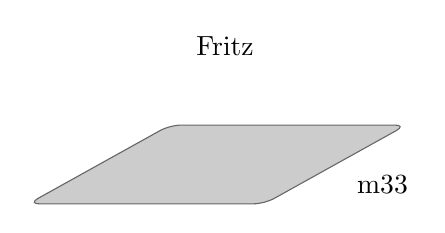
\begin{tikzpicture}[baseline=(fritz)]
  \begin{scope}[yshift=-1.5cm, xshift=-1.5cm, xslant=1.8]
    \filldraw [fill=black!20, draw=black!60, rounded corners] (0,0) rectangle (3,1);
  \end{scope}
  \Cat{black}
  \node (fritz) at (1,0.5) {Fritz};
  \node at (3,-1.25) {m33};
\end{tikzpicture}
\z
%
Since the record is of the type required by the record type -- which is represented in (\ref{ex:fritz-situation}) -- the type correctly classifies the situation in question.


\ea \label{ex:fritz-situation}
\begin{avm}
\[
x & = & Fritz \\
c1 & = & cat recognition \\
y & = & m33 \\
c2 & = & mat recognition \\
c3 & = & relation recognition
\]
\quad : \quad
\[
x & : & \ttrtype{Ind} \\
c1 & : & cat(x) \\
y & : & \ttrtype{Ind} \\
c2 & : & mat(y)  \\
c3 & : & on(x,y)
\]
\end{avm}
\z


Although record types will be represented in the above-given format, technically they involve functions \is{function} from individuals, not labels, to predicational types. 
%
That is, officially the \enquote{cat part} of the record type in (\ref{ex:fritz-situation}) has the following structure:
%
\ea \label{ex:official-notation}
\begin{avm}
\[
x & : & \ttrtype{Ind} \\
c1 & : & \<$\lambda v$:\ttrtype{Ind} . cat($v$), \q<x\q>\> 
\]
\end{avm}
\z
%
The predicational type c1 from (\ref{ex:official-notation}) is a function from individuals onto cats, i.e. it is of the Montagovian type $\langle e,t \rangle$, where the object abstracted over is to be found at path x in the record type. 
%
This function is characterised by the set of ordered pairs $\{\langle v, \ttrtype{cat}(v) \rangle \mid v : \ttrtype{Ind} \}$ and thereby is linked to a set theoretical notion of extension.
\is{type theory|)} \is{Type Theory with Records|)} \is{type-theoretical semantics|)}



\is{dialogue gameboard|(} \is{KoS|(}
\section{Putting things together: \HPSGTTR and Dialogue game boards}
\label{sec:hpsgttr-dialogue-game-boards}


Signs as construed within HPSG can be reconstructed as record types of a specific kind \citep{Cooper:2008}.
%
For instance, (\ref{ex:hpsgttr-sign}) shows the record type for a general \isi{sign} according to \citet{Pollard:Sag:1994} (where \ttrtype{PhonType}, \ttrtype{CategoryType} and \ttrtype{SemType} denote obvious types -- see the Appendix for a minimal HPSG fragment defined in terms of TTR).
%
\ea \label{ex:hpsgttr-sign}
\begin{avm}
\[
phon &:& \ttrtype{List}(\ttrtype{PhonType}) \\
synsem &:& 
    \[local &:&
        \[cat &:& \ttrtype{CategoryType} \\
        content &:& \ttrtype{SemType} \\
        context &:& \ttrtype{SemType}
        \]
    \]
\]
\end{avm}
\z

Signs are extended by an interface to \isi{circumstantial features} of the utterance situation in terms of the \textsc{dgb-params} \isfeat{dgb-params} attribute, which corresponds to the \textsc{c-inds} from Section~\ref{sec:c-inds-background}.
%
The attribute's name abbreviates \emph{dialogue gameboard parameters} \is{dialogue gameboard parameters} since its values have to be instantiated (that is, witnessed) \is{witness} in the process of \isi{grounding}.
%
Thus, if the content of an NP $\alpha$ is part of \textsc{dgb-params}, then $\alpha$ gets a \isi{referential interpretation}.
%
However, NPs need not be used referentially, there are descriptive uses \is{descriptive use} as in \textit{The thief (however he is) stole my credit card}.
%
To this end, there is a \enquote{coercion} operation from \textsc{dgb-params} to \textsc{q-params} \isfeat{q-params} (\emph{quantificational parameters}) \is{quantificational parameters} involving an abstraction from individuals to $\alpha$'s descriptive condition (\citet{Purver:Ginzburg:2004}; see the Appendix for the respective operation).


These \HPSGTTR signs figure as constituents within an architecture known as \emph{dialogue gameboard}, giving rise to a \isi{grammar-dialogue interface} within the dialogue theory \emph{KoS}
\citep{Ginzburg:1994,Ginzburg:1996,Ginzburg:2003,Ginzburg:2012}. 
%
A Dialogue Game Board (DGB) is an information-state based sheet for describing \isi{communicative interactions}.
%
The DGB from KoS tracks the interlocutors (\textit{spkr} and \textit{addr} fields), a record of the \isi{dialog history} (\textit{Moves}), dialog moves that are in the process of \isi{grounding} (\textit{Pending}), the question(s) currently under discussion \is{question under discussion} (\textit{QUD}), the assumptions shared among the interlocutors (\textit{Facts}), and   the dialogue
participant's view of 
the \isi{visual situation} and attended entities (\textit{VisualSit}).
%
\is{proposition|(} \is{Austinian proposition|(} \is{locutionary proposition|(}
The TTR representation of a DGB following \citet{Ginzburg:2012} is given in (\ref{ex:dgb}), where \textit{LocProp} is the type of a \emph{locutionary proposition} (see (\ref{ex:locprop}) below) and \textit{poset} abbreviates \enquote{partially ordered set}.
%
\ea \label{ex:dgb}
\begin{avm}
\[
spkr & : & \ttrtype{Ind} \\
addr & : & \ttrtype{Ind} \\
utt-time & : & \ttrtype{Time} \\
c-utt & : &  addressing(spkr, addr, utt-time) \\
facts & : & Set(\ttrtype{Prop}) \\
Visualsit & : & \ttrtype{RecType} \\
Pending & : & list(\ttrtype{LocProp}) \\
Moves & : & list(\ttrtype{LocProp}) \\
qud & : & poset(Question) \\
\]
\end{avm}
\z



Propositions in TTR can be developed in an explicit Austinian \aimention{John Langshaw Austin} (\citeyear{Austin:1950}) way, where a proposition is individuated in terms of a \isi{situation} and \isi{situation type} \citep[\page 845]{Ginzburg:2011:a} -- this is the truth-making (and Austin's original) interpretation of \enquote{It takes two to make a truth}.
%
The type of propositions and the relation to a situation semantics \is{situation semantic} conception of \enquote*{true} \citep{Barwise:Perry:1983} is given in (\ref{ex:propositions}):
%
\ea \label{ex:propositions}
\ea 
\begin{avm}
{\normalfont\ttrtype{Prop} $=_{\textit{def}}$} \[sit & : & \ttrtype{Record} \\ sit-type & : & \ttrtype{RecType}\]
\end{avm}
\ex 
\begin{avm}
{\normalfont A proposition $p =$}  \[sit & = & $s$ \\ sit-type & = & $T$\]\quad {\normalfont is true iff $s : T$}.
\end{avm}
\z
\z

A special kind of proposition, namely \emph{locutionary propositions} (\ttrtype{LocProp}) \citep[\page 172]{Ginzburg:2012}, can be defined as follows:
%
\ea \label{ex:locprop}
\begin{avm}
{\normalfont \ttrtype{LocProp} $=_{\textit{def}}$} \[sign & : & \ttrtype{Record} \\ sign-type & : & \ttrtype{RecType}\]
\end{avm}
\z
%
Locutionary propositions are sign objects utilized to explicate \isi{clarification potential} (see Section~\ref{sec:sub-sentential-meanings}) and \isi{grounding}. 
\is{proposition|(} \is{Austinian proposition|(} \is{locutionary proposition|(}

\is{interjections|(}
Given the dialogue-awareness of signs just sketched, a content for interjections such as \enquote{EHHH HEHH} which constitutes turn 3 from the exchange between Ann and Ray in (\ref{ex:ann-ray}) at the beginning of this chapter can be given.
%
Intuitively, Ann signals with these sounds that she heard Ray's question, which in turn is neither grounded nor clarified at this point of dialogue but waits for response, what is called \emph{pending}. \is{pending}
%
This intuition can be made precise by means of the following lexical entry (which is closely related to the meaning of \textit{mmh} given by \citet[\page 163]{Ginzburg:2012}):
%
\ea \label{ex:ehh-hehh}
\begin{avm}
\[
phon : ehh hehh \\
cat : \[head={\normalfont\ttrtype{interjection}} &:& \ttrtype{syncat}\] \\
dgb-params : \[spkr &:& \ttrtype{Ind} \\
              addr &:& \ttrtype{Ind} \\
              pending &:& \ttrtype{LocProp} \\
              c2 &:& address(spkr,addr,pending)
             \] \\
cont={\normalfont\ttrtype{Understand}}(spkr,addr,dgb-params.pending) : {\normalfont\ttrtype{IllocProp}}
\]
\end{avm}
\z

Knowing how  to use feedback signals \is{feedback} \is{feedback signal} such as the one in (\ref{ex:ehh-hehh}) can be claimed to be part of \isi{linguistic competence}.
%
It is difficult to imagine how to model this aspects of \isi{linguistic knowledge} if not by means of \emph{grammar in dialogue}.
\is{interjections|)}
\is{dialogue gameboard|)} \is{KoS|)}





\section{Outlook}
\label{sec:outlook-dialogue}

Given a basic framework for formulating and analysing content in dialogue context, there are various direction to explore, including the following ones.

\begin{itemize}
    \item 
One of the main challenges of dialogue semantics is the integration of \emph{non-verbal communication} means, like gaze, gestures, body posture, timing and non-language  vocal sounds (e.g., laughter \citep{Ginzburg:Breitholz:Cooper:Hough:Tian:2015,Tian:Mazzocconi:Ginzburg:2016}).
%
Since \isi{non-verbal communication} means are informative, not only a (dialogue) semantic representation has to be developed, but also the rules of their interaction with speech has to be formulated. 

\item Duologue \is{duologue} is the interaction between \emph{two} interlocutors. 
%
How can one scale up to \emph{multilogue} \is{multilogue} \citep{Ginzburg:Fernandez:2005}?
%
Given the increased number of participants,  problems that emerge include  \emph{grounding by proxy}, \is{grounding} where a representative represents the dialogue gameboard of a group and of course \emph{turn taking}.

\item People do not process natural language input sentence-wise.
%
Rather, processing begins with the initial sound and proceeds word for word or even on smaller units like morphemes and phonemes -- that is, processing is incremental \is{incremental} \is{incremental processing} (e.g. \citet{Sedivy:Tanenhaus:Chambers:Carlson:1999}; see also \crossrefchaptert{processing}). This is a key ingredient in the efficient (relatively gap-free and interruption-less) managing of turn taking.
%
One direction of dialogue theories therefore is to bring psycholinguistics and formal semantics closer together by devising incremental grammar and dialogue gameboard models \citep{Hough:Kennington:Schlangen:Ginzburg:2015,Demberg:Keller:Koller:2013,Poesio:Rieser:2011}.

\end{itemize}


Finally, we want to mention two other dialogue-theoretic frameworks that have been worked out to a substantial degree, namely \isi{PTT} \citep{Traum:1994,Poesio:1995,Poesio:Traum:1997,Poesio:Rieser:2010}, and \emph{Segmented Discourse Representation Theory} \is{Segmented Discourse Representation Theory} (SDRT) \citep{Asher:1993,Asher:Lascarides:2003,Asher:Lascarides:2013,Hunter:Asher:2015}.
%
The phenomena and outlook directions discussed in this chapter apply to all theories of dialogue semantics, of course. 




\is{HPSG-TTR|(}
%\appendix
\section*{Appendix: A \HPSGTTR fragment}

The appendix provides a fragment of \HPSGTTR.
%
The grammar framework used is oriented at a \textit{Head-driven Phrase Structure Grammar} variant \citep{Sag:Wasow:Bender:2003}, respectively its TTR implementation \citep{Cooper:2008}.
%
We use HPSG, because its  architecture satisfies the property of \emph{incremental correspondence} \citep{Johnson:Lappin:1999} -- utterance representations encode phonological, syntactic, semantic, and contextual information \emph{fractally}.
%
 This is crucial {\it inter alia} for any treatment of clarification interaction (cf. Section~\ref{sec:sub-sentential-meanings}). 
%
We use HPSG\textsubscript{TTR}, because the type-theoretical version allows us to directly incorporate semantic objects (cf. Section~\ref{sec:semantic-objects}).


TTR has a counterpart to unification, namely the \emph{merge} construction.
%
\ea
\ea If $R_1$ and $R_2$ are record types, then $R_1 \ttrmerge R_2$ is a record type and is called the \emph{merge} of $R_1$ and $R_2$.
\ex Since merge types are complicated to define \citep[but see][]{Cooper:2012}, we follow the strategy of \citet{Cooper:2017:a} and illustrate the working of merges by means of some examples:
\begin{enumerate}[label=(\roman*), leftmargin=6.5em]
\item 
\begin{avm}
\[a &:& $T$ \\ b &:& $R$\]
\quad\ttrmerge\space\space
\[c &:& $S$\]
\quad = \space
\[a &:& $T$ \\ b &:& $R$ \\ c &:& $S$\]
\end{avm}
%%
\item 
\begin{avm}
\[a &:& $T$ \]
\quad\ttrmerge\space\space
\[a &:& $R$ \]
\quad = \space
\[a &:& $T$ \ttrmerge\ $R$\]
\end{avm}
\end{enumerate}
\z
\z


Structure sharing is indicated by a \enquote{tag type} notation.
%
Tag type are defined in terms of manifest fields.\footnote{\textit{NB:} technically, tag types apply singleton types to record types, instead of to objects, thereby making use of a revision of the notion of singleton types introduced by \citet[\pno~4, footnote~3]{Cooper:2013}.}
%
The notational convention is exemplified in (\ref{ex:tag-notation}) by means of head-specifier agreement, where the tag type from (\ref{ex:tag-notation}a) abbreviates the structure in (\ref{ex:tag-notation}b):
%
\ea \label{ex:tag-notation}
\ea
\begin{avm}
\[
cat &:& \[head &:& \[agr$_{\@{1}}$ &:& \ttrtype{Agr}\] \\
          spr &:& \<[cat &:& \[head &:& \[agr=\@{1} &:& \ttrtype{Agr}\]\]\>
        \]
\]
\end{avm}
\ex 
\begin{avm}
\[
cat &:& \[head &:& \[agr &:& \ttrtype{Agr}\] \\
          spr &:& \<[cat &:& \[head &:& \[agr=/cat.head.agr &:& \ttrtype{Agr}\]\]\>
        \]
\]
\end{avm}
\z
\z 
%
The tag type notation alludes to the box notation common in HPSG work.


\ttrtype{Agr} is defined as usual:
%
\ea
\ttrtype{Agr} $\coloneqq$
\begin{avm}
\[num &:& \ttrtype{Num} \\
pers &:& \ttrtype{Per} \\
gen &:& \ttrtype{Gen}
\]
\end{avm}
\z 

% The grammar framework makes use of some grammar-specific types, which are enumerated (partly employing obvious abbreviations) in the following:
% %
% \begin{itemize}
% \item Parts of speech: \ttrtype{noun}, \ttrtype{verb}, \ttrtype{prep} \ldots of type \ttrtype{PoS};
% %%
% \item Type of constituent: \ttrtype{lexeme}, \ttrtype{word}, \ttrtype{phrase};
% %%
% \item Number: \ttrtype{sg}, \ttrtype{pl} of type \ttrtype{Num};
% %%
% \item Person: \ttrtype{1st}, \ttrtype{2nd}, \ttrtype{3rd} of type \ttrtype{Pers};
% %%
% \item Gender: \ttrtype{fem}, \ttrtype{masc}, \ttrtype{neut} of type \ttrtype{Gend};
% %%
% \item Case: \ttrtype{nom}, \ttrtype{acc}, \ttrtype{gen}, \ttrtype{dat} of type \ttrtype{Case};
% %%
% \item A type \ttrtype{Phoneme} which captures phonetic representations (which are simplified in terms of orthographic transcriptions);
% %%
% \item Semantic objects: \ttrtype{Ind}, \ttrtype{Quant}, \ttrtype{Prop}, \ttrtype{Set}(\ttrtype{Ind}), \ldots\ of type \ttrtype{SemObj} (see  \textcite{Ginzburg:2012} for more on \ttrtype{SemObj});
% %%
% \item The type \ttrtype{SynCat} takes care of syntactic information and includes fixed path names like \enquote{head}, \enquote{spr} (specifier), \enquote{comps} (complements);
% %%
% \end{itemize}


A basic \emph{sign} is a pairing of phonetic, syntactic and semantic information and follows the geometry in (\ref{ex:sign}): 
%
\ea \label{ex:sign}
\ttrtype{sign} $\coloneqq$ 
\begin{avm}
\[
phon &:& \ttrtype{Phoneme} \\
cat &:& \ttrtype{SynCat} \\
dgb-params &:& \ttrtype{RecType} \\
cont &:& \ttrtype{SemObj} \\
\]
\end{avm}
\z

Signs employ dgb-params, which host referential meanings that are witnessed among interlocutors. 
%
Quantificational abstraction is achieved by coercing parts of dgb-params to q-params:
%
\ea
If dgb-params : $R_2$ and for two record types $R_0$ and $R_1$ lacking any mutual dependencies\footnote{None of the labels occurring in $R_0$ occur in $R_1$ and vice versa.}
$R_2 = R_0 \wedge_{merge} R_1$,
 % $R_0 \sqsubseteq R_1$
then $R_0$ can be moved to q-params, resulting in the following structure: \par\medskip 
 % \commentrhc{You should explain what you mean by $\setminus$. We would need an example to make sure this is working. }
 
\begin{avm}
\[
dgb-params &:& $R_1$\\
%\setminus R_0$ \\
cont &=& \[q-params &:& $R_0$\]
\]
\end{avm}
\z



A word is a sign with constituent type (\enquote{cxtype}) \ttrtype{word}.
%
Using the merge operation, the word extension on signs can represented compactly as in (\ref{ex:word}a), which expands to the structure given in (\ref{ex:word}b):
%

\ea \label{ex:word}
\ea \ttrtype{word} $\coloneqq$ \ttrtype{sign} \ttrmerge\ \begin{avm}
\[cxtype &:& \ttrtype{word}\]
\end{avm} : \ttrtype{RecType}
\ex 
\begin{avm}
\[
cxtype &:& \ttrtype{word} \\
phon &:& \ttrtype{Phoneme} \\
cat &:& \ttrtype{SynCat} \\
dgb-params &:& \ttrtype{RecType} \\
cont &:& \ttrtype{SemObj} 
\]
\end{avm}
\z
\z

Words -- that is, cxtype \ttrtype{word} -- are usually the result of lexical rules, whose input are lexemes.
%
Lexemes differ from words in their constituent type:
%
\ea
\ttrtype{lexeme} $\coloneqq$ \ttrtype{sign} \ttrmerge\ \begin{avm}
\[cxtype &:& \ttrtype{lexeme}\]
\end{avm} : \ttrtype{RecType}
\z

A phrasal sign can be seen as a word with daughters:
%
\ea 
\ea \ttrtype{phrase} $\coloneqq$ \ttrtype{sign} \ttrmerge\ \begin{avm}
\[cxtype &:& \ttrtype{phrase} \\
dtrs &:& \[nhd-dtrs &:& \ttrtype{List}(\ttrtype{Sign})\]\]
\end{avm} : \ttrtype{RecType}
\ex 
\begin{avm}
\[
cxtype &:& \ttrtype{phrase} \\
phon &:& \ttrtype{List}(\ttrtype{Phoneme}) \\
cat &:& \ttrtype{SynCat} \\
dgb-params &:& \ttrtype{RecType} \\
cont &:& \ttrtype{SemObj} \\
dtrs &:& \[% hd-dtr &:& \ttrtype{Sign} \\
           nhd-dtrs &:& \ttrtype{List}(\ttrtype{Sign})
         \]
\]
\end{avm}
\z
\z

A headed phrase is a phrase with a prominent daughter, i.e., the head daughter:
%
\ea 
\ea \ttrtype{hd-phrase} $\coloneqq$ \ttrtype{phrase} \ttrmerge\ 
\begin{avm}
\[dtrs &:& \[hd-dtr &:& \ttrtype{Sign}\]\]
\end{avm} : \ttrtype{RecType}
\ex 
\begin{avm}
\[
cxtype &:& \ttrtype{phrase} \\
phon &:& \ttrtype{List}(\ttrtype{Phoneme}) \\
cat &:& \ttrtype{SynCat} \\
dgb-params &:& \ttrtype{RecType} \\
cont &:& \ttrtype{SemObj} \\
dtrs &:& \[hd-dtr &:& \ttrtype{Sign} \\
           nhd-dtrs &:& \ttrtype{List}(\ttrtype{Sign})
         \]
\]
\end{avm}
\z
\z

The head daughter is special since it (as a default at least) determines the syntactic properties of the mother construction. 
%
This aspect of headedness is captured in terms of the \emph{head-feature principle} (HFP), which can be implemented by means of tag types as follows:
%
\ea \label{ex:HFP}
HFP $\coloneqq$
\begin{avm}
\[
cxtype &:& \ttrtype{phrase} \\
cat &:& \[head$_{\@{2}}$ &:& \ttrtype{PoS}\] \\
dtrs &:& \[hd-dtr &:& \[cat &:& \[head=\@{2} &:& \ttrtype{PoS}\]\] \\
         \]
\]
\end{avm}
\z

The fact that the daughters' locutions combine to the mother's utterance is captured in terms of a \enquote{phon principle}  (we use a slash notation in order to indicate paths starting at the outermost level of a feature structure):
%
\ea 
PHON $\coloneqq$ \label{ex:phon-principle}
\begin{avm}
\[
cxtype &:& \ttrtype{phrase} \\
phon &:& \ttrtype{List}(/dtrs.hd.dtr/phon, /dtrs.nhd.dtrs/pos1.phon,  \\ && \ldots, /dtrs.nhd.dtrs/pos$n$.phon) 
% dtrs &:& \[hd-dtr &:& \ttrtype{Sign} \\
%           nhd-dtrs &:& \ttrtype{List}(\ttrtype{Sign})
%         \]
\]
\end{avm}
\z 

Since  semantic composition rests on predication rather than unification, there is no analog to the semantic compositionality principle of \citet{Sag:Wasow:Bender:2003} on our account.
%
There is, however, something akin to semantic inheritance: we need to keep track of the contextual resp. quantificational paramaters contributed by the daughters of a phrase. 
%
This is achieved in terms of a \emph{dgb-params principle} (\ttrtype{DGBPP}) in (\ref{ex:dgbpp}) which unifies the daughters' dgb-params into the mother's dgb-params  (see \citet[126 \textit{et seq.}]{Ginzburg:2012}  for a similar principle): 
%
\ea \label{ex:dgbpp}
DGBPP $\coloneqq$ \label{ex:QPP} \par\medskip
\oneline{%
\begin{avm}
\[
cxtype &:& \ttrtype{phrase} \\
dgb-params &:& \[/dtrs.hd-dtr.dgb-params\ \ttrmerge\ /dtrs.nhd-dtrs.pos1.dgb-params\ \ttrmerge \\ \ldots \ttrmerge\ /dtrs.nhd-dtrs.pos$n$.dgb-params
             \] \\
dtrs &:& \[hd-dtr &:& \[q-params &:& \ttrtype{RecType}\] \\
           nhd-dtrs &:& \<pos1 &:& \[q-params &:& \ttrtype{RecType}\],  
                         \ldots, 
                         pos$n$ &:& \[q-params &:& \ttrtype{RecType}\]
                        \>
         \]
\]
\end{avm}
}
\z

A headed phrase is well-formed just in case it is a headed phrase and it obeys the head feature principle, the phon principle and the dgb-params principle, which is expressed by extending \ttrtype{hd-phrase} by the following constraint:
%
\ea \label{ex:hd-phrase}
\ttrtype{hd-phrase} $\coloneqq$ 
\ttrtype{hd-phrase} \ttrmerge\ {HFP} \ttrmerge\  {PHON} \ttrmerge\ {DGBPP}
\z


Using this set-up, lexical entries, lexical rules and syntactic constructions can be formulated straightforwardly. 
\is{HPSG-TTR|)}
 
% \section*{Abbreviations}
% \section*{Acknowledgements}

%\avmoptions{active}

}% end avmoptions

{\sloppy
  \printbibliography[heading=subbibliography,notkeyword=this] 
}
\end{document}
